% ------------------------------------------------------------------------------
% TYPO3 CMS 7.1 - What's New (Dutch Version)
%
% @author	Michael Schams <schams.net>
% @license	Creative Commons BY-NC-SA 3.0
% @link		http://typo3.org/download/release-notes/whats-new/
% @language	Dutch
% ------------------------------------------------------------------------------
% LTXE-CHAPTER-UID:		e7264f0e-3f82290d-94c50cda-fb2d8e66
% LTXE-CHAPTER-NAME:	Gebruikersinterface backend
% ------------------------------------------------------------------------------

\section{Gebruikersinterface backend}
\begin{frame}[fragile]
	\frametitle{Gebruikersinterface backend}

	\begin{center}\huge{Hoofdstuk 1:}\end{center}
	\begin{center}\huge{\color{typo3darkgrey}\textbf{Gebruikersinterface backend}}\end{center}

\end{frame}

% ------------------------------------------------------------------------------
% LTXE-SLIDE-START
% LTXE-SLIDE-UID:		4353aa2a-3c9e854e-d62e2008-7fd171ff
% LTXE-SLIDE-ORIGIN:	d5fddde9-b3ee31c0-f0509300-40a2928e English
% LTXE-SLIDE-TITLE:		Date/Time Picker
% LTXE-SLIDE-REFERENCE:	Breaking-62925-RemoveExtJsDateTimePicker.rst
% ------------------------------------------------------------------------------

\begin{frame}[fragile]
	\frametitle{Gebruikersinterface backend}
	\framesubtitle{Look \& Feel: Datum/Tijd Kiezer}

	Datum/Tijd Kiezer is vervangen door een Bootstrap-alternatief
	\begin{figure}
		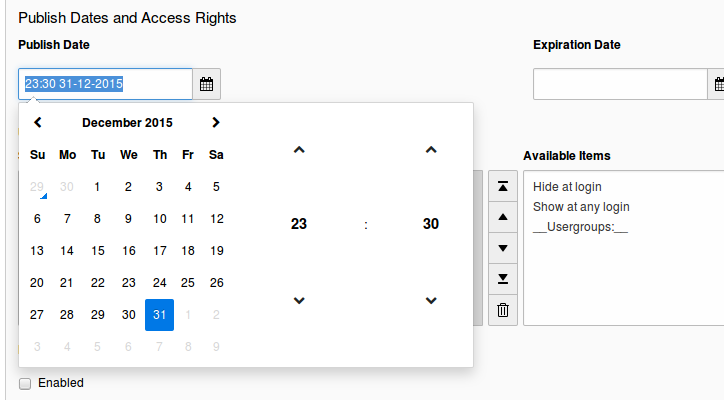
\includegraphics[width=0.75\linewidth]{BackendUserInterface/be-datepicker.png}
	\end{figure}

\end{frame}

% ------------------------------------------------------------------------------
% LTXE-SLIDE-START
% LTXE-SLIDE-UID:		9f9ebb1e-60e0b66b-3973903b-80defe8c
% LTXE-SLIDE-ORIGIN:	1c391eec-dfb1dfa6-f783ae7a-d0b214ae English
% LTXE-SLIDE-TITLE:		Functions Module
% LTXE-SLIDE-REFERENCE:	Breaking-63310-Wizard-Modules-Moved.rst
% ------------------------------------------------------------------------------

\begin{frame}[fragile]
	\frametitle{Gebruikersinterface backend}
	\framesubtitle{Look \& Feel: Functiemodules}

	"Pagina's aanmaken" en "Pagina's sorteren" verplaatst: \texttt{Web => Functies}\newline
	\smaller (in TYPO3 CMS < 7.1 waren deze te vinden onder "\texttt{Web => Functies => Wizards}")

	\begin{figure}
		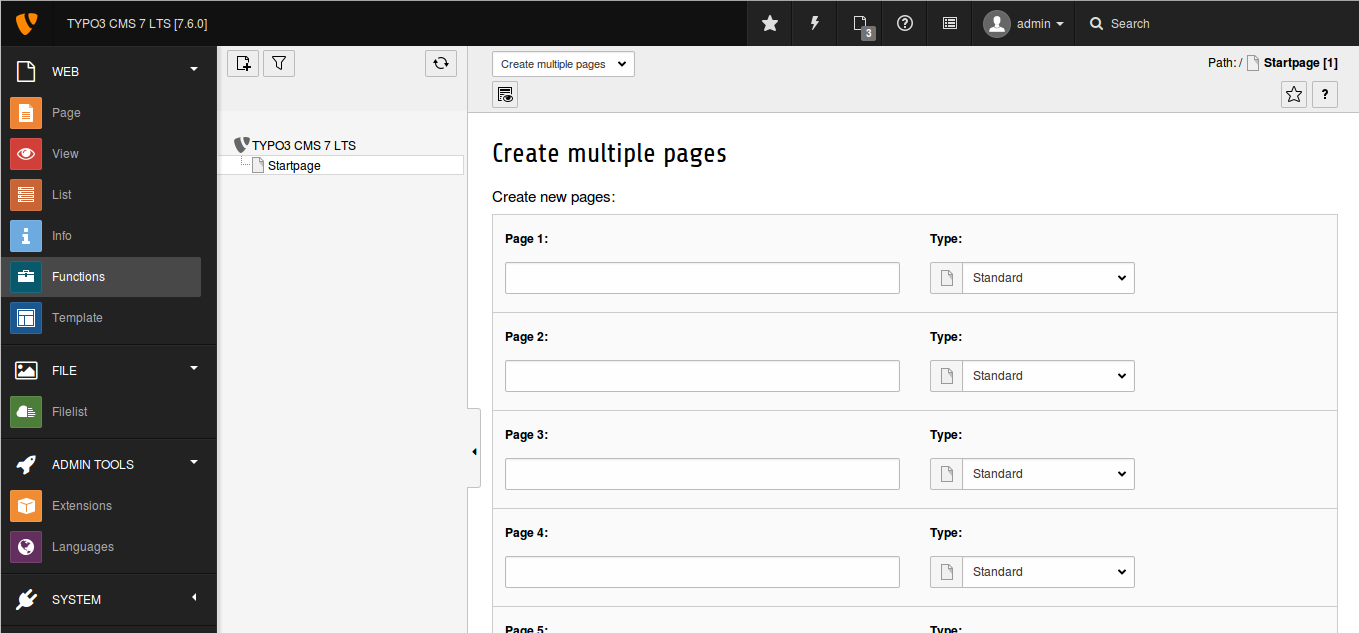
\includegraphics[width=0.80\linewidth]{BackendUserInterface/be-functions.png}
	\end{figure}


\end{frame}

% ------------------------------------------------------------------------------
% LTXE-SLIDE-START
% LTXE-SLIDE-UID:		ee0d36cf-12c01db3-49b74177-7dea193d
% LTXE-SLIDE-ORIGIN:	dd127630-5ccc729a-835e5836-e8796962 English
% LTXE-SLIDE-TITLE:		Access Module: Leave Unchaged
% LTXE-SLIDE-REFERENCE:	Feature-15619-LeaveUnchagedInAccessModule.rst
% ------------------------------------------------------------------------------

\begin{frame}[fragile]
	\frametitle{Gebruikersinterface backend}
	\framesubtitle{Look \& Feel: Toegangsmodule}

	Module \texttt{Web => Toegang} maakt het nu mogelijk om gebruikers/groepen ongewijzigd
	te laten bij het overschrijven van permissies

	\begin{figure}
		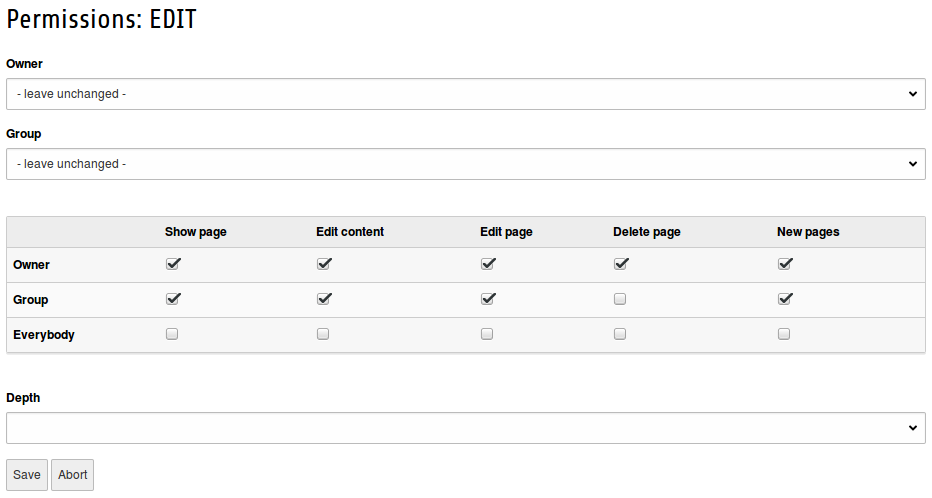
\includegraphics[width=0.75\linewidth]{BackendUserInterface/be-access.png}
	\end{figure}

\end{frame}

% ------------------------------------------------------------------------------
% LTXE-SLIDE-START
% LTXE-SLIDE-UID:		e3e13b68-ee34971b-651bdaa6-cb063c46
% LTXE-SLIDE-ORIGIN:	eb6cc867-e4f5d0d3-ea06672c-7ccdf227 English
% LTXE-SLIDE-TITLE:		Icons in List Module
% LTXE-SLIDE-REFERENCE:	Feature-63207-SplitActionButtonsIntoGroups.rst
% ------------------------------------------------------------------------------

\begin{frame}[fragile]
	\frametitle{Gebruikersinterface backend}
	\framesubtitle{Look \& Feel: Iconen in Lijstmodule}

	Iconen ("actie knoppen") in de lijstweergave is verdeeld in twee groepen\newline
	\smaller (primaire acties eerst (lezen, bijwerken, verwijderen), gevolgd door secondaire acties)

	\begin{figure}
		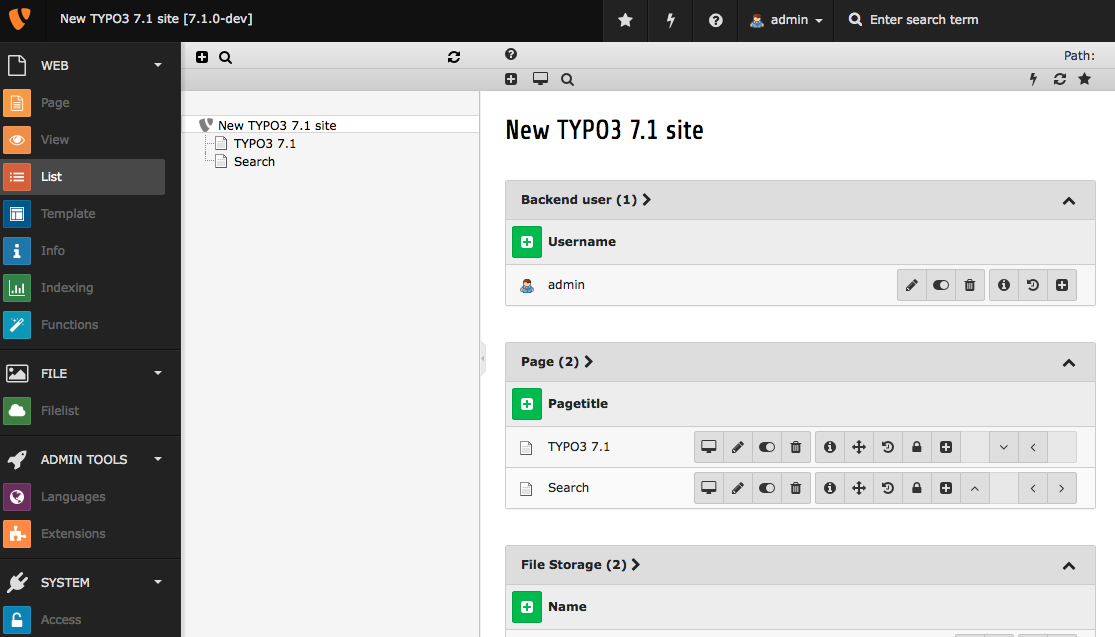
\includegraphics[width=0.75\linewidth]{BackendUserInterface/be-icons.png}
	\end{figure}

\end{frame}

% ------------------------------------------------------------------------------
